% !TeX root = ../main.tex
% Add the above to each chapter to make compiling the PDF easier in some editors.

\chapter{Evaluation}\label{chapter:evaluation}
\section{Tasks to evaluate}

\subsection{Evaluation of the completeness and accuracy of the produced heuristics against a reference data set}
To evaluate the completeness and accuracy of the heuristics produced during the development of this thesis a reference data set has been used.\\
We implemented a procedure to check all files in the projects whether it contains a generator-pattern. These files are separately saved in a list and reviewed randomly for their amount of false positives. \\
Bernwieser~\cite{Bernwieser2014} provided a list of files that he detected as generated to us, to witch our results are compared against. \\
We do this to evaluate whether the approach given in this thesis is an improvement to the existing ones, especially the one given by~\cite{Bernwieser2014}. It resolves whether the generator-pattern repository can be used as a database in production while performing static code analysis.

\subsection{Automatic classification of source code in a huge collection of open source systems \& evaluation of the ratio of generated code}
To test the generator patterns stored in the repository a variety of open source projects have been acquired.\\
These projects have been filtered using the generator-pattern repository to detect the amount of generated code in a huge, randomly composed collection of open source systems.\\
We calculated the amount of generated code in these projects to evaluate the usage of code generators and their importance in programming. 

\section{Study Objects}
We used different study objects to test the approach used in this thesis and to evaluate the completeness and accuracy of the generator-pattern repository. \\
A reference data set is described in Section~\ref{section:qualitasCorpus} which includes good documented code, whereas Section~\ref{section:randomGitProjects} describes a randomly composed collection of open source projects that is used to test the generator-pattern repository in a not particularly curated environment.
 
\subsection{Qualitas Corpus}
\label{section:qualitasCorpus}
"The Qualitas Corpus is a curated collection of software systems intended to be used for empirical studies of code artefacts. The primary goal is to provide a resource that supports reproducible studies of software. The current release of the Corpus contains open-source Java software systems, often multiple versions." \cite{TemperoEwanandAnslowCraigandDietrichJensandHanTedandLiJingandLumpeMarkusandMeltonHaydenandNoble2010a}\\
Nonetheless the procedure is designed to be also applicable onto sets including other programming languages as well as sets of projects with mixed ones.\\
The current release is from the year 2013 and includes 112 different projects. To be easily comparable to the work in \cite{Bernwieser2014}, we also added the project Mahout~\cite{ApacheSoftwareFoundation}.\\
Additionally, we could perform the analysis on all projects so we didn't have to exclude \textit{eclipse\_SDK} nor \textit{netbeans}.\\
Table~\ref{table:qualitasCorpusAll} displays all projects that are included in the Qualitas Corpus together with their amount of lines of code. The size of the projects ranges from 6.991 \textit{(fitjava)} up to 7.142.778 \textit{(netbeans)}.
% !TeX root = ../main.tex
% Add the above to each chapter to make compiling the PDF easier in some editors.
\setlength{\extrarowheight}{-0.02em}
\begin{table}
	\caption{All projects of the Qualitas Corpus and their respective lines of code.}
	\label{table:qualitasCorpusAll}
	\begin{tabularx}{\textwidth}{c|c||c|c||C|c}
		\textbf{Project} & \textbf{LOC} & \textbf{Project} & \textbf{LOC} & \textbf{Project} & \textbf{LOC} \\
		\hline
		ant & 256.041 & antlr & 58.935 & aoi & 153.186 \\
		argouml & 389.952 & aspectj & 598.485 & axion & 41.862 \\
		azureus & 831.586 & batik & 366.507 & c\_jdbc & 174.972 \\
		castor & 349.301 & cayenne & 341.902 & checkstyle & 89.922 \\
		cobertura & 68.154 & collections & 109.415 & colt & 84.592 \\
		columba & 149.498 & compiere & 727.702 & derby & 1.138.858 \\
		displaytag & 38.729 & drawswf & 46.540 & drjava & 160.308 \\
		eclipse\_SDK & 4.956.920 & emma & 39.676 & exoportal & 146.947 \\
		findbugs & 185.806 & fitjava & 6.991 & fitlibraryforfitnes & 42.233 \\
		freecol & 205.085 & freecs & 29.943 & freemind & 86.244 \\
		galleon & 135.442 & ganttproject & 69.322 & gt2 & 1.514.789 \\
		hadoop & 444.593 & heritrix & 126.652 & hibernate & 711.370 \\
		hsqldb & 269.978 & htmlunit & 174.415 & informa & 29.587 \\
		ireport & 338.819 & itext & 145.118 & ivatagroupware & 71.851 \\
		jag & 28.957 & james & 83.716 & jasml & 7.272 \\
		jasperreports & 347.502 & javacc & 35.145 & jboss & 968.808 \\
		jchempaint & 372.743 & jedit & 176.672 & jena & 164.679 \\
		jext & 100.210 & jFin\_DateMath & 16.686 & jfreechart & 313.268 \\
		jgraph & 59.145 & jgraphpad & 43.652 & jgrapht & 41.887 \\
		jgroups & 137.614 & jhotdraw & 133.830 & jmeter & 182.552 \\
		jmoney & 11.304 & joggplayer & 51.654 & jparse & 32.270 \\
		jpf & 22.521 & jrat & 31.084 & jrefactory & 301.940 \\
		jruby & 244.774 & jspwiki & 110.005 & jstock & 74.361 \\
		jsXe & 35.307 & jtopen & 645.715 & jung & 67.024 \\
		junit & 13.359 & log4j & 68.612 & lucene & 611.422 \\
		mahout & 177.325 & marauroa & 36.859 & maven & 111.581 \\
		megamek & 336.267 & mvnforum & 172.855 & myfaces\_core & 189.954 \\
		nakedobjects & 214.777 & nekohtml & 13.342 & netbeans & 7.142.778 \\
		openjms & 111.837 & oscache & 19.702 & picocontainer & 15.999 \\
		pmd & 80.971 & poi & 363.487 & pooka & 72.167 \\
		proguard & 101.330 & quartz & 62.229 & quickserver & 30.239 \\
		quilt & 13.035 & roller & 135.210 & rssowl & 174.209 \\
		sablecc & 35.388 & sandmark & 128.993 & springframework & 624.388 \\
		squirrel\_sql & 9.082 & struts & 261.537 & sunflow & 27.408 \\
		tapestry & 182.151 & tomcat & 352.572 & trove & 9.768 \\
		velocity & 70.804 & wct & 99.622 & webmail & 18.074 \\
		weka & 496.737 & xalan & 354.578 & xerces & 237.555 \\
		& & xmojo & 43.249 & &
	\end{tabularx}
\end{table}
\setlength{\extrarowheight}{0em}

\subsection{Random Git Projects}
\label{section:randomGitProjects}
To collect a huge, randomly composed collection of open source projects a git crawler has been implemented.
By passing a keyword to the crawler it queries \href{github.com}{GitHub} to return project descriptions of projects that contain the keyword in their names or descriptions. From the received project descriptions the links to clone the projects are extracted. The projects are cloned and saved sorted by their programming languages, whereas the crawler queries for projects written in all languages supported by Teamscale to provide the highest level of randomness and diversity for the projects.
% !TeX root = ../main.tex
% Add the above to each chapter to make compiling the PDF easier in some editors.
\setlength{\extrarowheight}{.5em}
\begin{table}
	\caption[Overview over the open source projects.]{The distribution of projects on the respective programming languages and their lines of code for the collection of open source projects.}
	\label{table:gitProjects}
	\begin{tabularx}{\textwidth}{c|r|r|c|r|r|c|r|r}
		\textbf{Lang.} & \textbf{\#} & \textbf{LOC} &\textbf{Lang.} & \textbf{\#} & \textbf{LOC} &\textbf{Lang.} & \textbf{\#} & \textbf{LOC} \\
		ABAP & 10 & 55.498 &
		Ada & 5 & 194.961 &
		C & 145 & 4.791.612 \\
		COBOL & 3 & 58.968 &
		Delphi & 3 & 15.470 &
		Gosu & 6 & 2.738 \\
		Groovy & 66 & 143.939 &
		Java & 230 & 4.879.454 &
		JavaScript & 138 & 6.828.723 \\
		Kotlin & 58 & 87.132 &
		Matlab & 30 & 134.229 &
		OScript & 122 & 2.837.202 \\
		PHP & 68 & 1.016.013 &
		Python & 133 & 858.223 &
		Rust & 35 & 1.248.308 \\
		Swift & 55 & 457.629 &
		XML & 13 & 28.541 &
		\textbf{Total} & \textbf{1122} & \textbf{23.638.640}
		
	\end{tabularx}
\end{table}
\setlength{\extrarowheight}{0em}

\section{Study Design}
To evaluate the completeness and accuracy of the produced heuristics we used the Qualitas Corpus to calculate the amount of generated code. Using this information we compared our results to the ones provided in \cite{Bernwieser2014} to derive the improvement our approach makes in distinguishing generated from manually maintained code.\\
Based on the set of generated source code files we calculated different metrics:
\begin{itemize}
	\item Lines of code for generated and manually maintained source code.
	\item Number of generated and manually maintained source code files.
	\item Ratio of lines of code per source code files in the categories.
\end{itemize}

\section{Procedure}
This section justifies the decisions we made for the different thresholds as well as our decision to highly multithread the different steps used in the approach.

\subsection{Testing environment}
The benchmarks are performed on an \href{https://www.intel.de/}{\textit{Intel Core i7-6700HQ CPU}} running with a frequency of \textit{2.60GHz} on \textit{four} physical cores with \textit{40GB RAM}. To run the Java Code we used the \href{https://www.eclipse.org/}{\textit{Eclipse IDE}} executed on \href{https://www.ubuntu.com/}{\textit{Ubuntu 18.04.1 LTS (64-bit)}} based on the \href{https://www.ubuntu.com/}{\textit{4.15.0-33-generic} Kernel}.\\
We compare the durations of the single steps performed during the suffix-tree clone-detection approach to find generator-patterns. We used the projects \textit{azureus, batik, checkstyle, cobertura, compiere, derby, drjava, exoportal, freecol, freecs, galleon, hsqldb, htmlunit, ireport, ivatagroupware, jFin\_DateMath, javacc, jedit, jgrapht, jhotdraw, jmoney, joggplayer, jparse, jspwiki, jstock, jung, maven, netbeans, openjms, oscache, quilt, sandmark, squirrel\_sql, tapestry, trove, weka, xerces} as a reference benchmark environment and ran the procedure several times to calculate a solid average value for the durations. \\
The decision for this environment is reasoned by its size of 37~projects including 60.235~source code files, whereas 3034~files are generated. It contains a total of 1.166.654~comments with a total of 23.683.887~valuable words. This pushes the machine the benchmark has been performed on to its maximum heap space it can provide to the Java Virtual Machine. The projects are chosen randomly to provide a meaningful mean of projects to preserve the generality of the Qualitas Corpus.

\subsection{Thresholds}
The threshold that has a direct impact on the number of found generator-patterns is the minimum clone length. It describes the minimal length a sequence of \code{CloneChunk}s has to provide to be considered by the Step~\ref{section:findClones}. If a sequence is shorter than the minimum clone length it will not be added to the list of clone classes independent of the size the clone class would have.\\
Finding the best minimum clone length has been done by performing tests with different clone lengths ranging from a length of 2\footnote{We didn't start at 1 because single words aren't meaningful when searching for generator-patterns. Especially words like \textit{the, a, by \dots} would have many occurrences that generate a huge amount of false positive clone classes.} up to a length of 25.\\
We finally decided on the minimum clone length of 5, where as the choice has been a mostly subjective one. Nonetheless did we consider the draw-off between the amount of results that are lost due to a to high minimum clone length and the amount of irrelevant data generated by a to low minimum clone length.\\
Figure~\ref{fig:thresholdsAll} shows all found \code{CloneResult}s associated to the minimum clone length used to find it. It can be seen that by increasing the minimum clone length the number of \code{CloneResult}s drops nearly exponentially. \\
After applying the processing steps described in Step~\ref{section:processCloneResults} to reduce the amount of data that is created, the remaining \code{CloneResult}s behave as shown in Figure~\ref{fig:thresholdsProcessed}. It shows that by filtering the amount of \code{CloneResult}s drops by around 99\%, dropping even further by accumulating and clustering.\\
We tried using the minimum clone length of 3 at first due to the peak in the remaining \code{CloneResult}s. Nonetheless did we decide to use 5 because the observation was that no generator-patterns were lost by using this minimum clone length, but the manual search for the patterns in the links was much easier because the sequences were more meaningful.
% !TeX root = ../../main.tex
% Add the above to each chapter to make compiling the PDF easier in some editors.

\begin{figure}
	\centering
	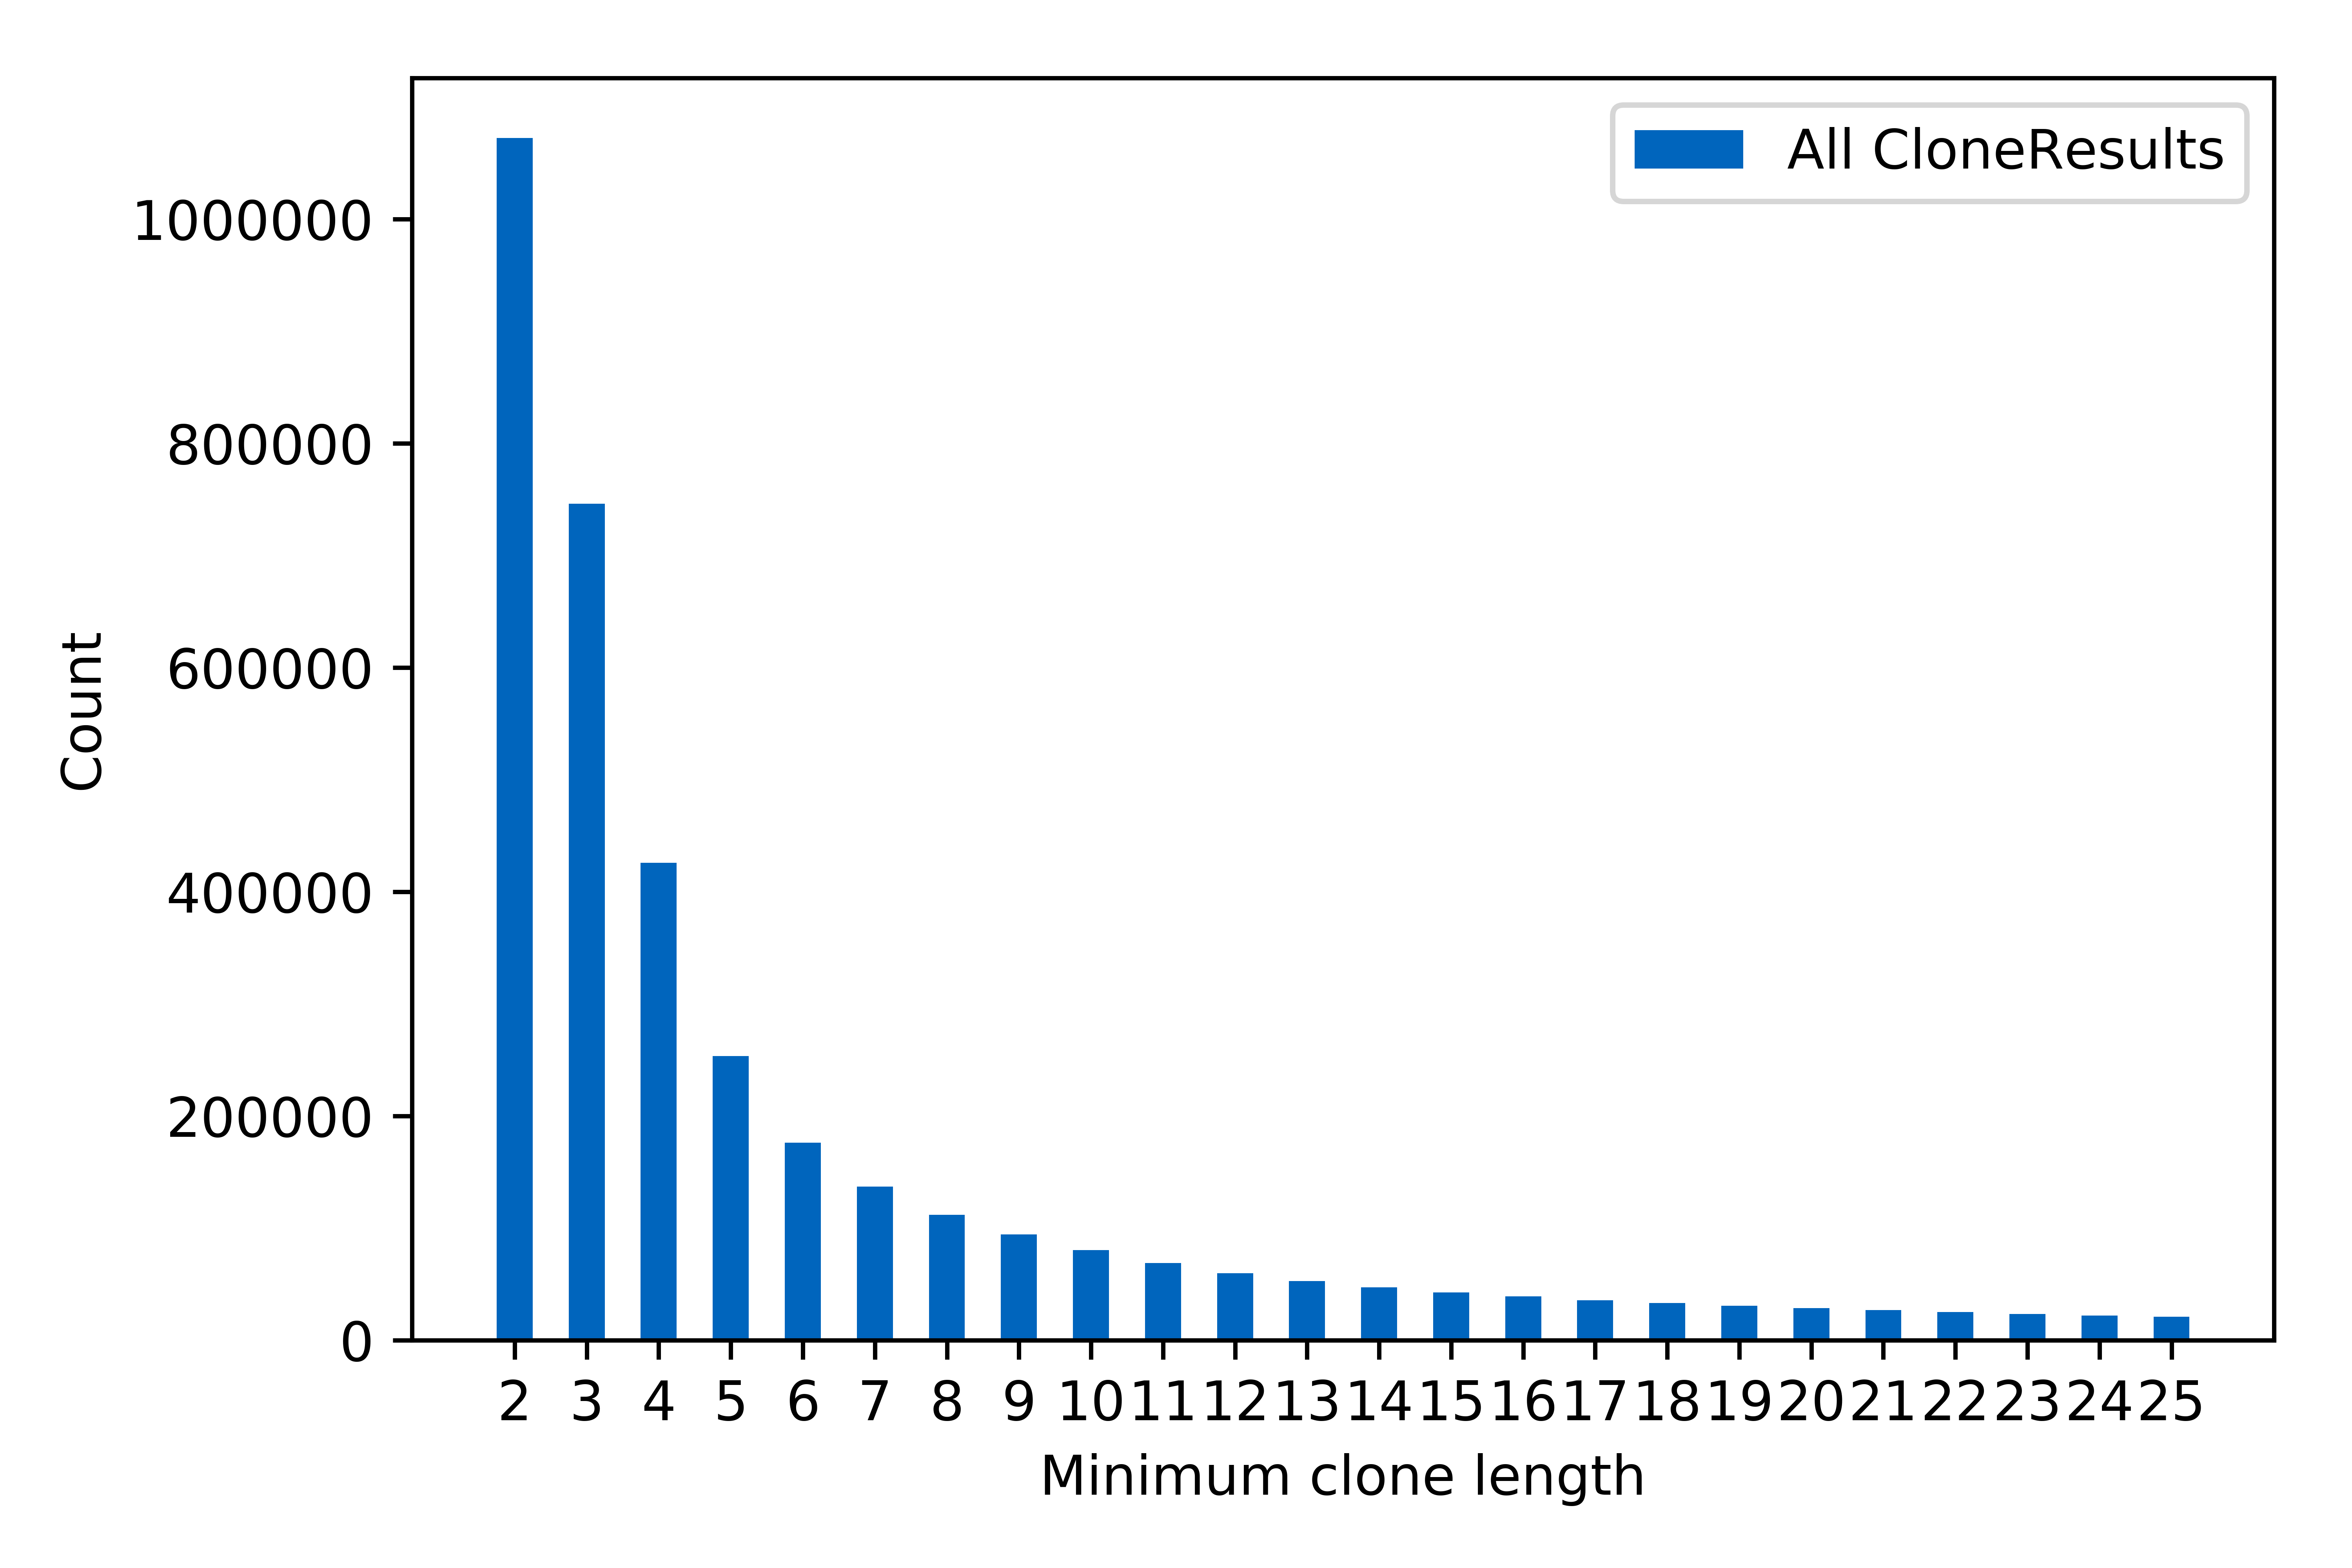
\includegraphics[width=0.8\linewidth]{figures/Thresholds/raw.png}
	\caption[All found Cloneclasses in relation to the minimum clone length]{This chart shows the number of \code{CloneResult}s found by the suffix-tree clone-detection in relation to the minimum clone length used to find them.}
	\label{fig:thresholdsAll}
\end{figure}

% !TeX root = ../../main.tex
% Add the above to each chapter to make compiling the PDF easier in some editors.

\begin{figure}
	\centering
	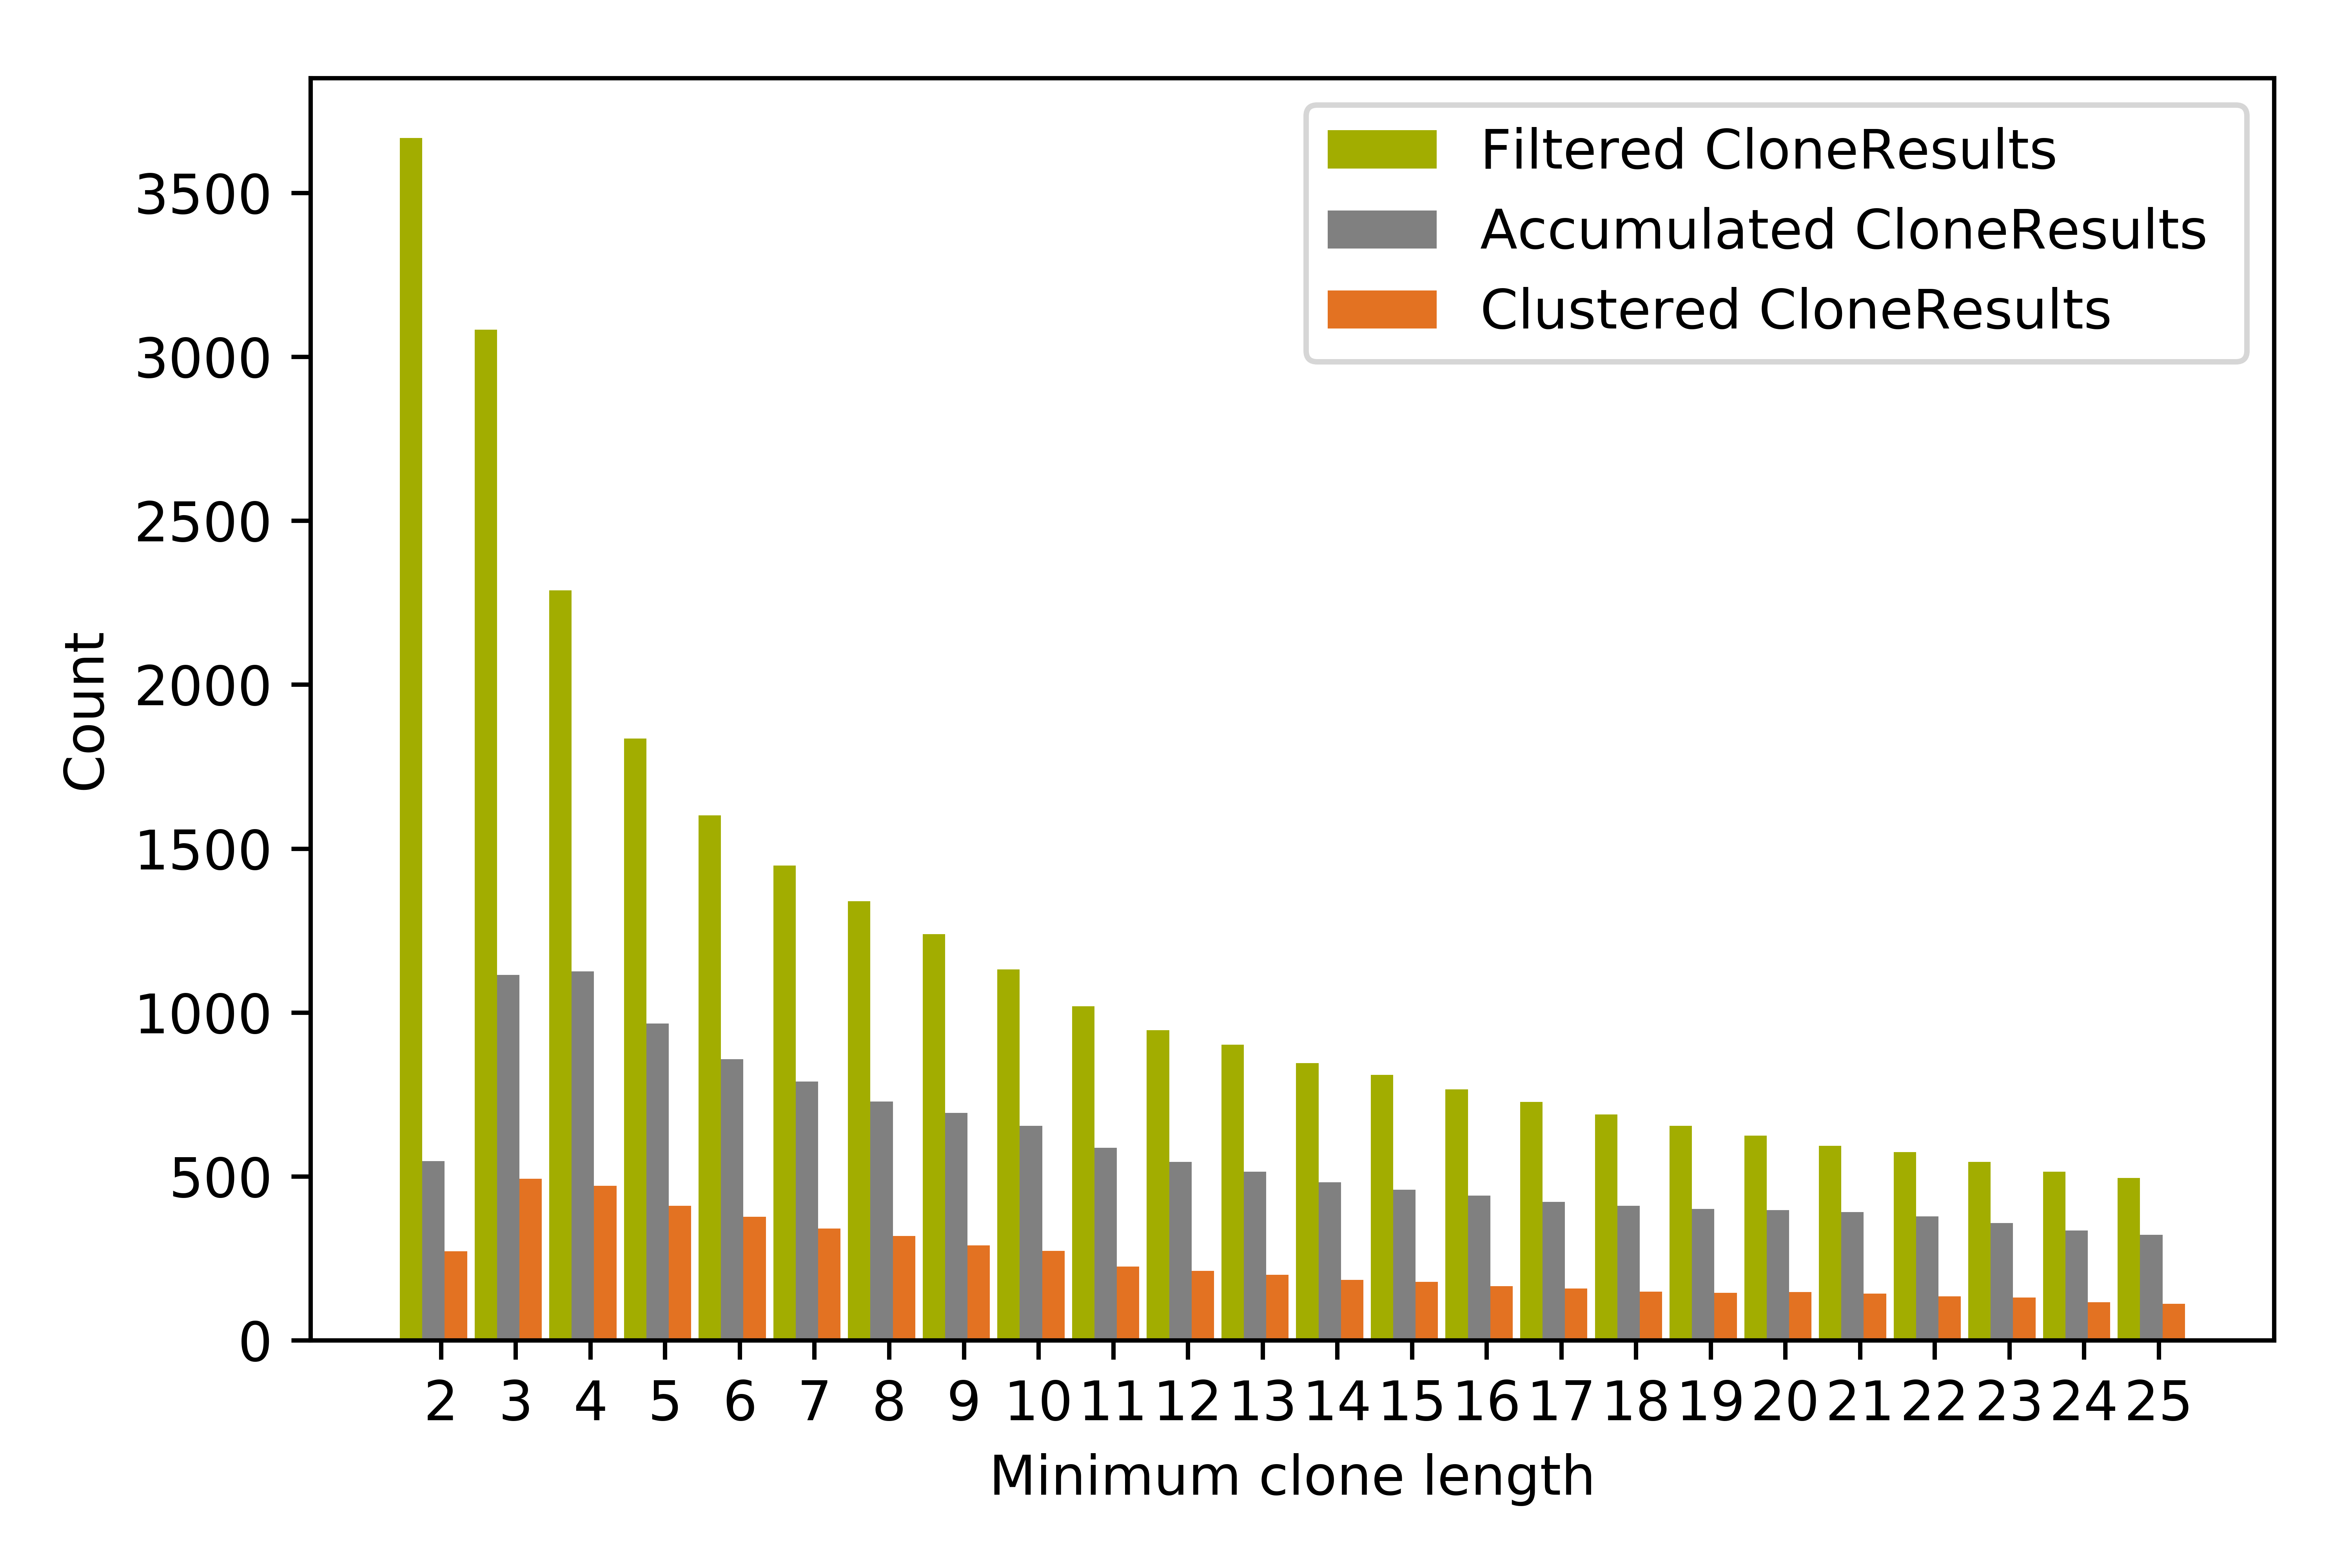
\includegraphics[width=0.8\linewidth]{figures/Thresholds/processed.png}
	\caption[Processed CloneClasses in relation to the minimum clone length]{This chart shows the number of \code{CloneResult}s that are left after the three processing steps described in Step~\ref{section:processCloneResults}. The counts are associated to their respective minimum clone length used to find the \code{CloneResult}s.}
	\label{fig:thresholdsProcessed}
\end{figure}


\subsection{Benchmarking}
\label{section:benchmark}
As displayed in Figure~\ref{fig:benchmark}, the time-intensive steps are multithreaded.\\
We performed the benchmark with a minimum clone length of 5.\\
This results in time savings ranging from 5.32\% \textit{(Get Uniform Paths)} up to 86.25\% \textit{(Create Links For: GENERATED)}. The overall time saving sums up to a total of 56.5\%, which reduces the average absolute amount of time of around 300 seconds down to 130 seconds. 
% !TeX root = ../../main.tex
% Add the above to each chapter to make compiling the PDF easier in some editors.
\begin{figure}
	\centering
	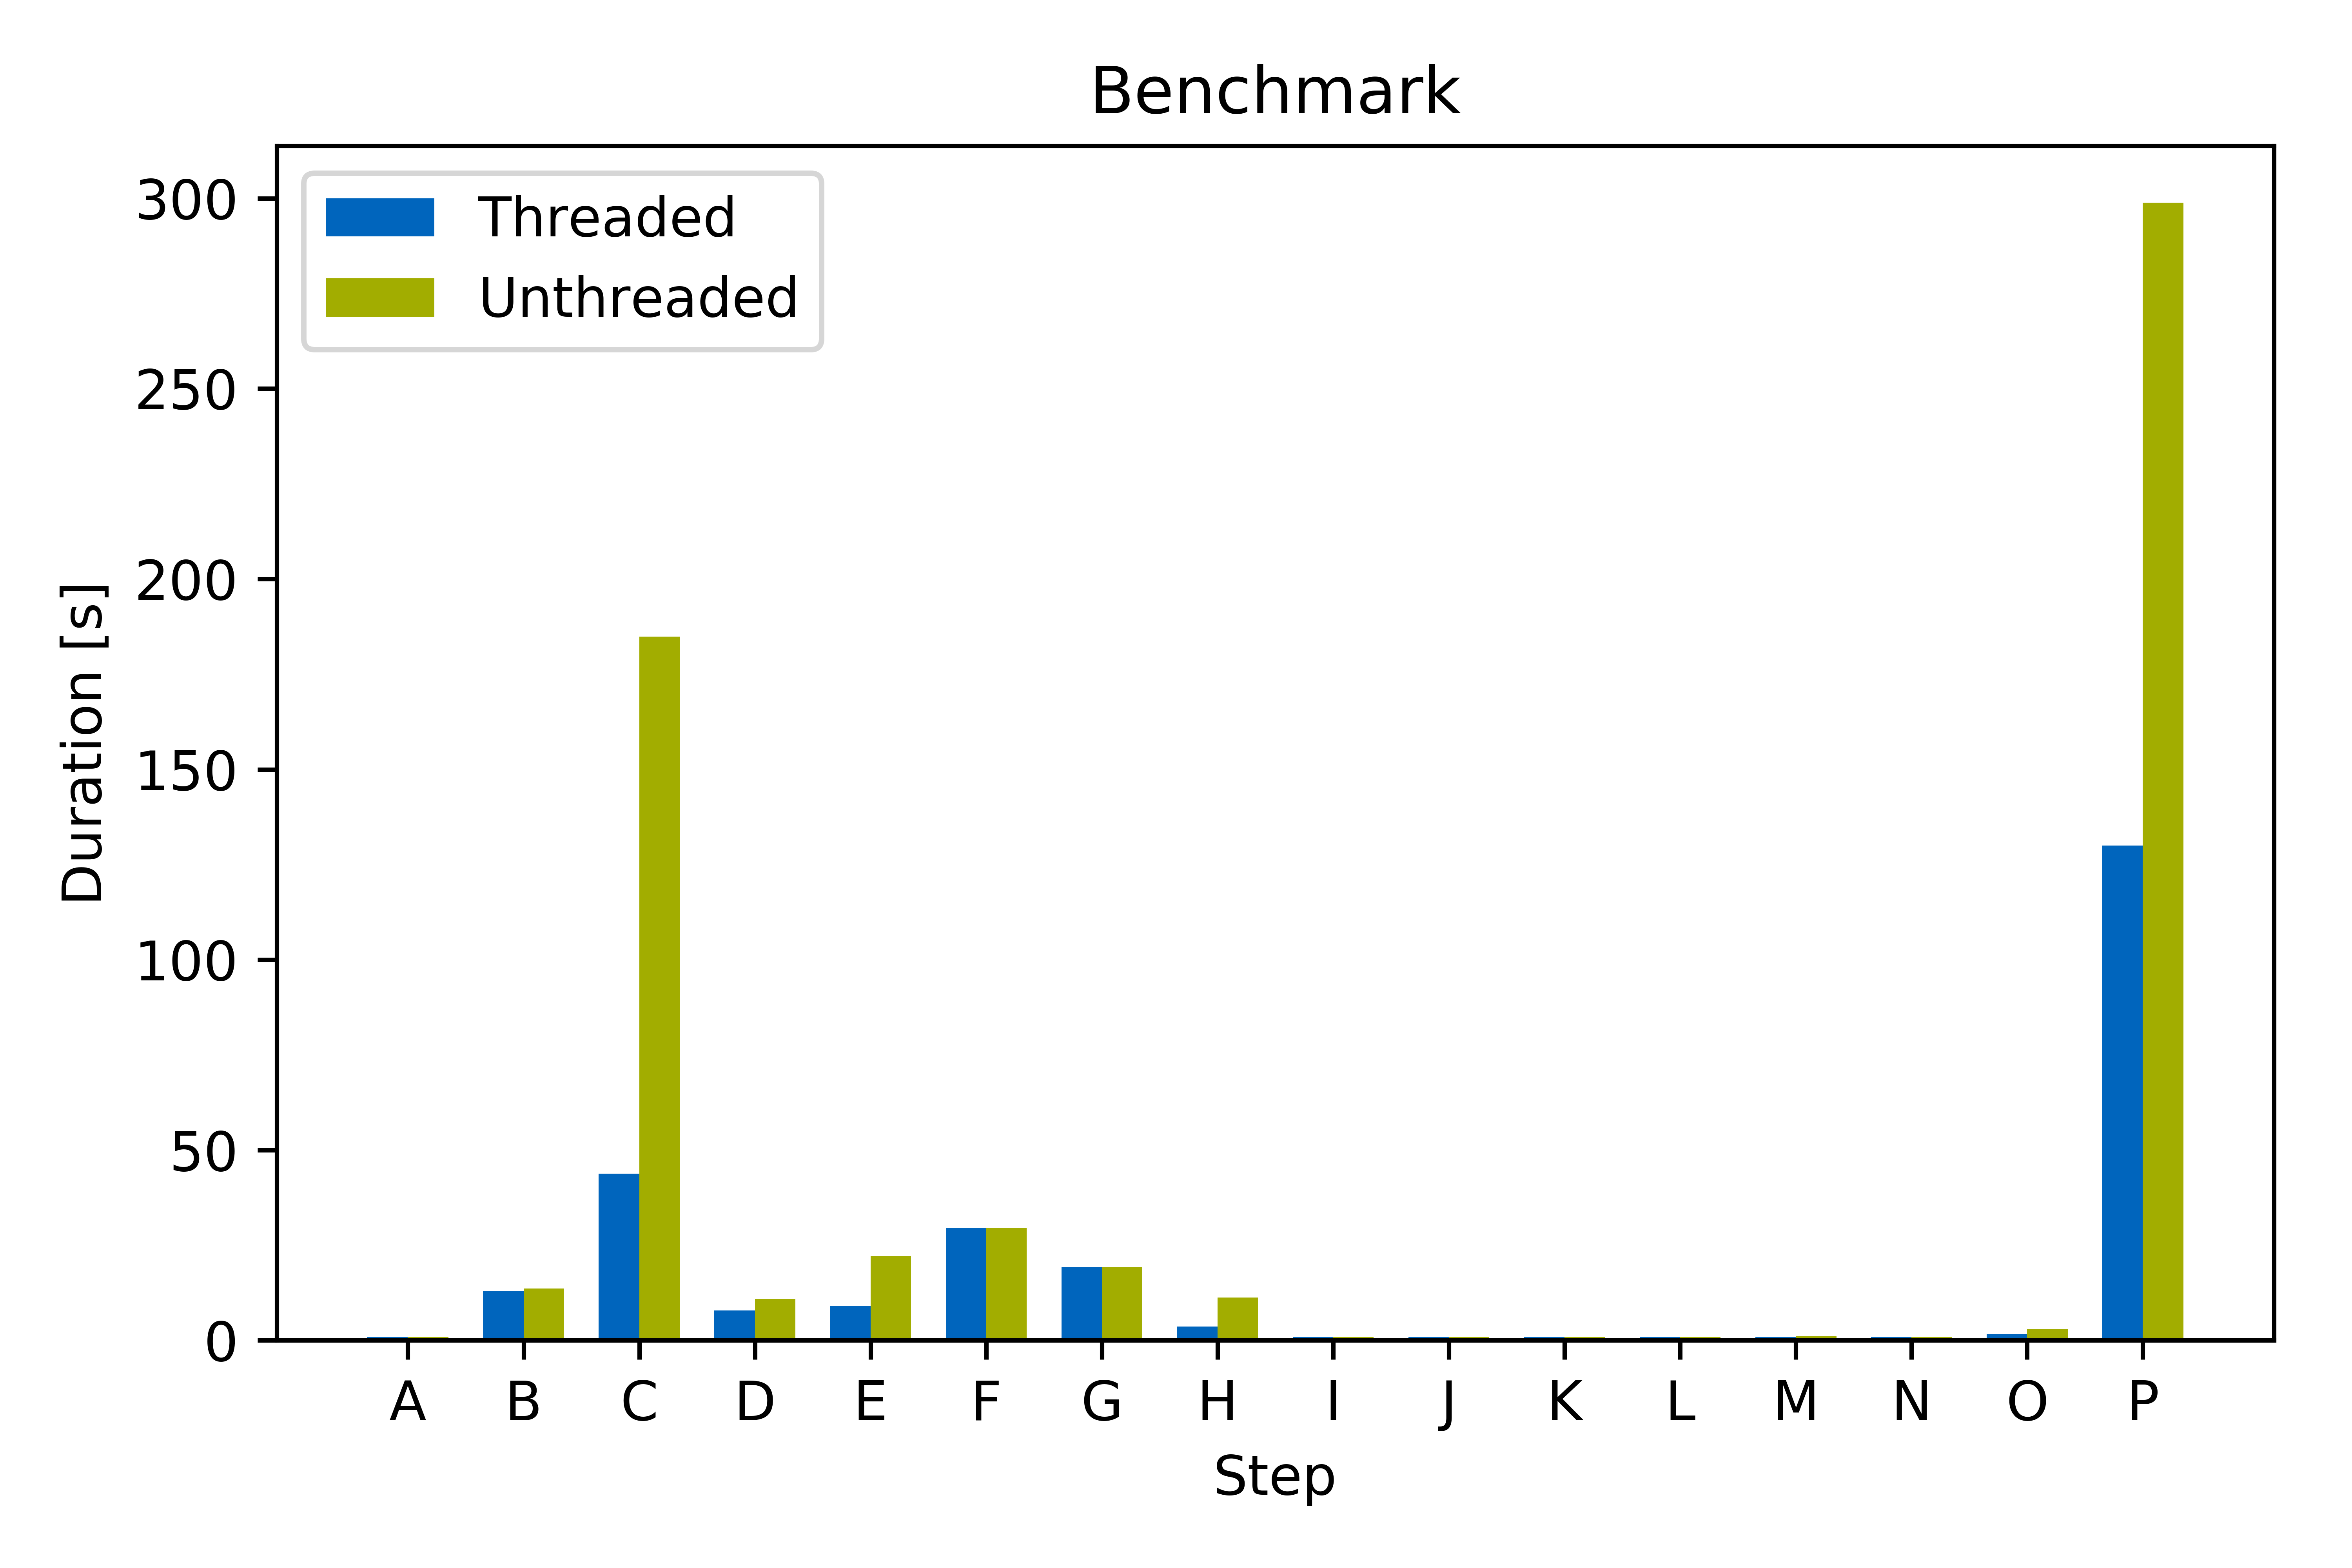
\includegraphics[width=0.8\linewidth]{figures/Benchmark/benchmark.png}
	\caption[Benchmark]{The results of the benchmarks performed during the search for generator-patterns. The step labels are explained in Table~\ref{table:tickLabels}.}
	\label{fig:benchmark}
\end{figure}
% !TeX root = ../main.tex
% Add the above to each chapter to make compiling the PDF easier in some editors.
\setlength{\extrarowheight}{.0em}
\begin{table}
	\caption{Explanation for the step labels of Figure~\ref{fig:benchmark}. The \textit{Savings} column displays the time saving gained through multithreading.}
	\label{table:tickLabels}
		\begin{tabularx}{\textwidth}{c|C|c||c|C|c}
			\textbf{Tick} & \textbf{Step} & \textbf{Savings} & \textbf{Tick} & \textbf{Step} & \textbf{Savings}\\
			\hline
			A & Get Projects & - & B & Get Uniform Paths & 5.32\% \\
			C & Retrieve Comments & 76.29\% & D & Save Comments & 27.78\% \\
			E & Prepare Comments & 59.29\% &F& Build Suffix Tree & - \\
			G& Find Clones & - & H & Convert to \code{CloneResult}s & 67.54\%\\
			I&Filter Presumable Generator Patterns & - &J&Accumulate Presumable Generator Patterns & -\\
			K&Cluster Presumable Generator Patterns & - &L&Filter Presumable Not Generator Patterns & -\\
			M& Save Files For: GENERATED& 83.06\% &N&Create Links For: GENERATED & 86.25\%\\
			O& Create Links For: NOT\_GENERATED& 42.41\% & P & Total & 56.5\%
		\end{tabularx}
\end{table}
\setlength{\extrarowheight}{0em}

\section{Results}
This section displays the results we were able to create by using the approach to find generator-patterns and by using the the resulting generator-pattern repository on the different data sets. 
\subsection{Qualitas Corpus}
At first we considered the Qualitas Corpus because it provided a good database and the results can be compared to the ones made in \cite{Bernwieser2014}.\\
We found a total of 41 from the 112 projects to contain generated code. 

\subsubsection{Number of generator-patterns found}
A total of 48 generator-patterns have been found. They are generated by 29 different generators. Additionally most of the patterns are regular expressions that accept up to 32 different patterns so that the final number of found generator patterns is much higher.

%% !TeX root = ../../main.tex
% Add the above to each chapter to make compiling the PDF easier in some editors.

\begin{figure}
	\centering
	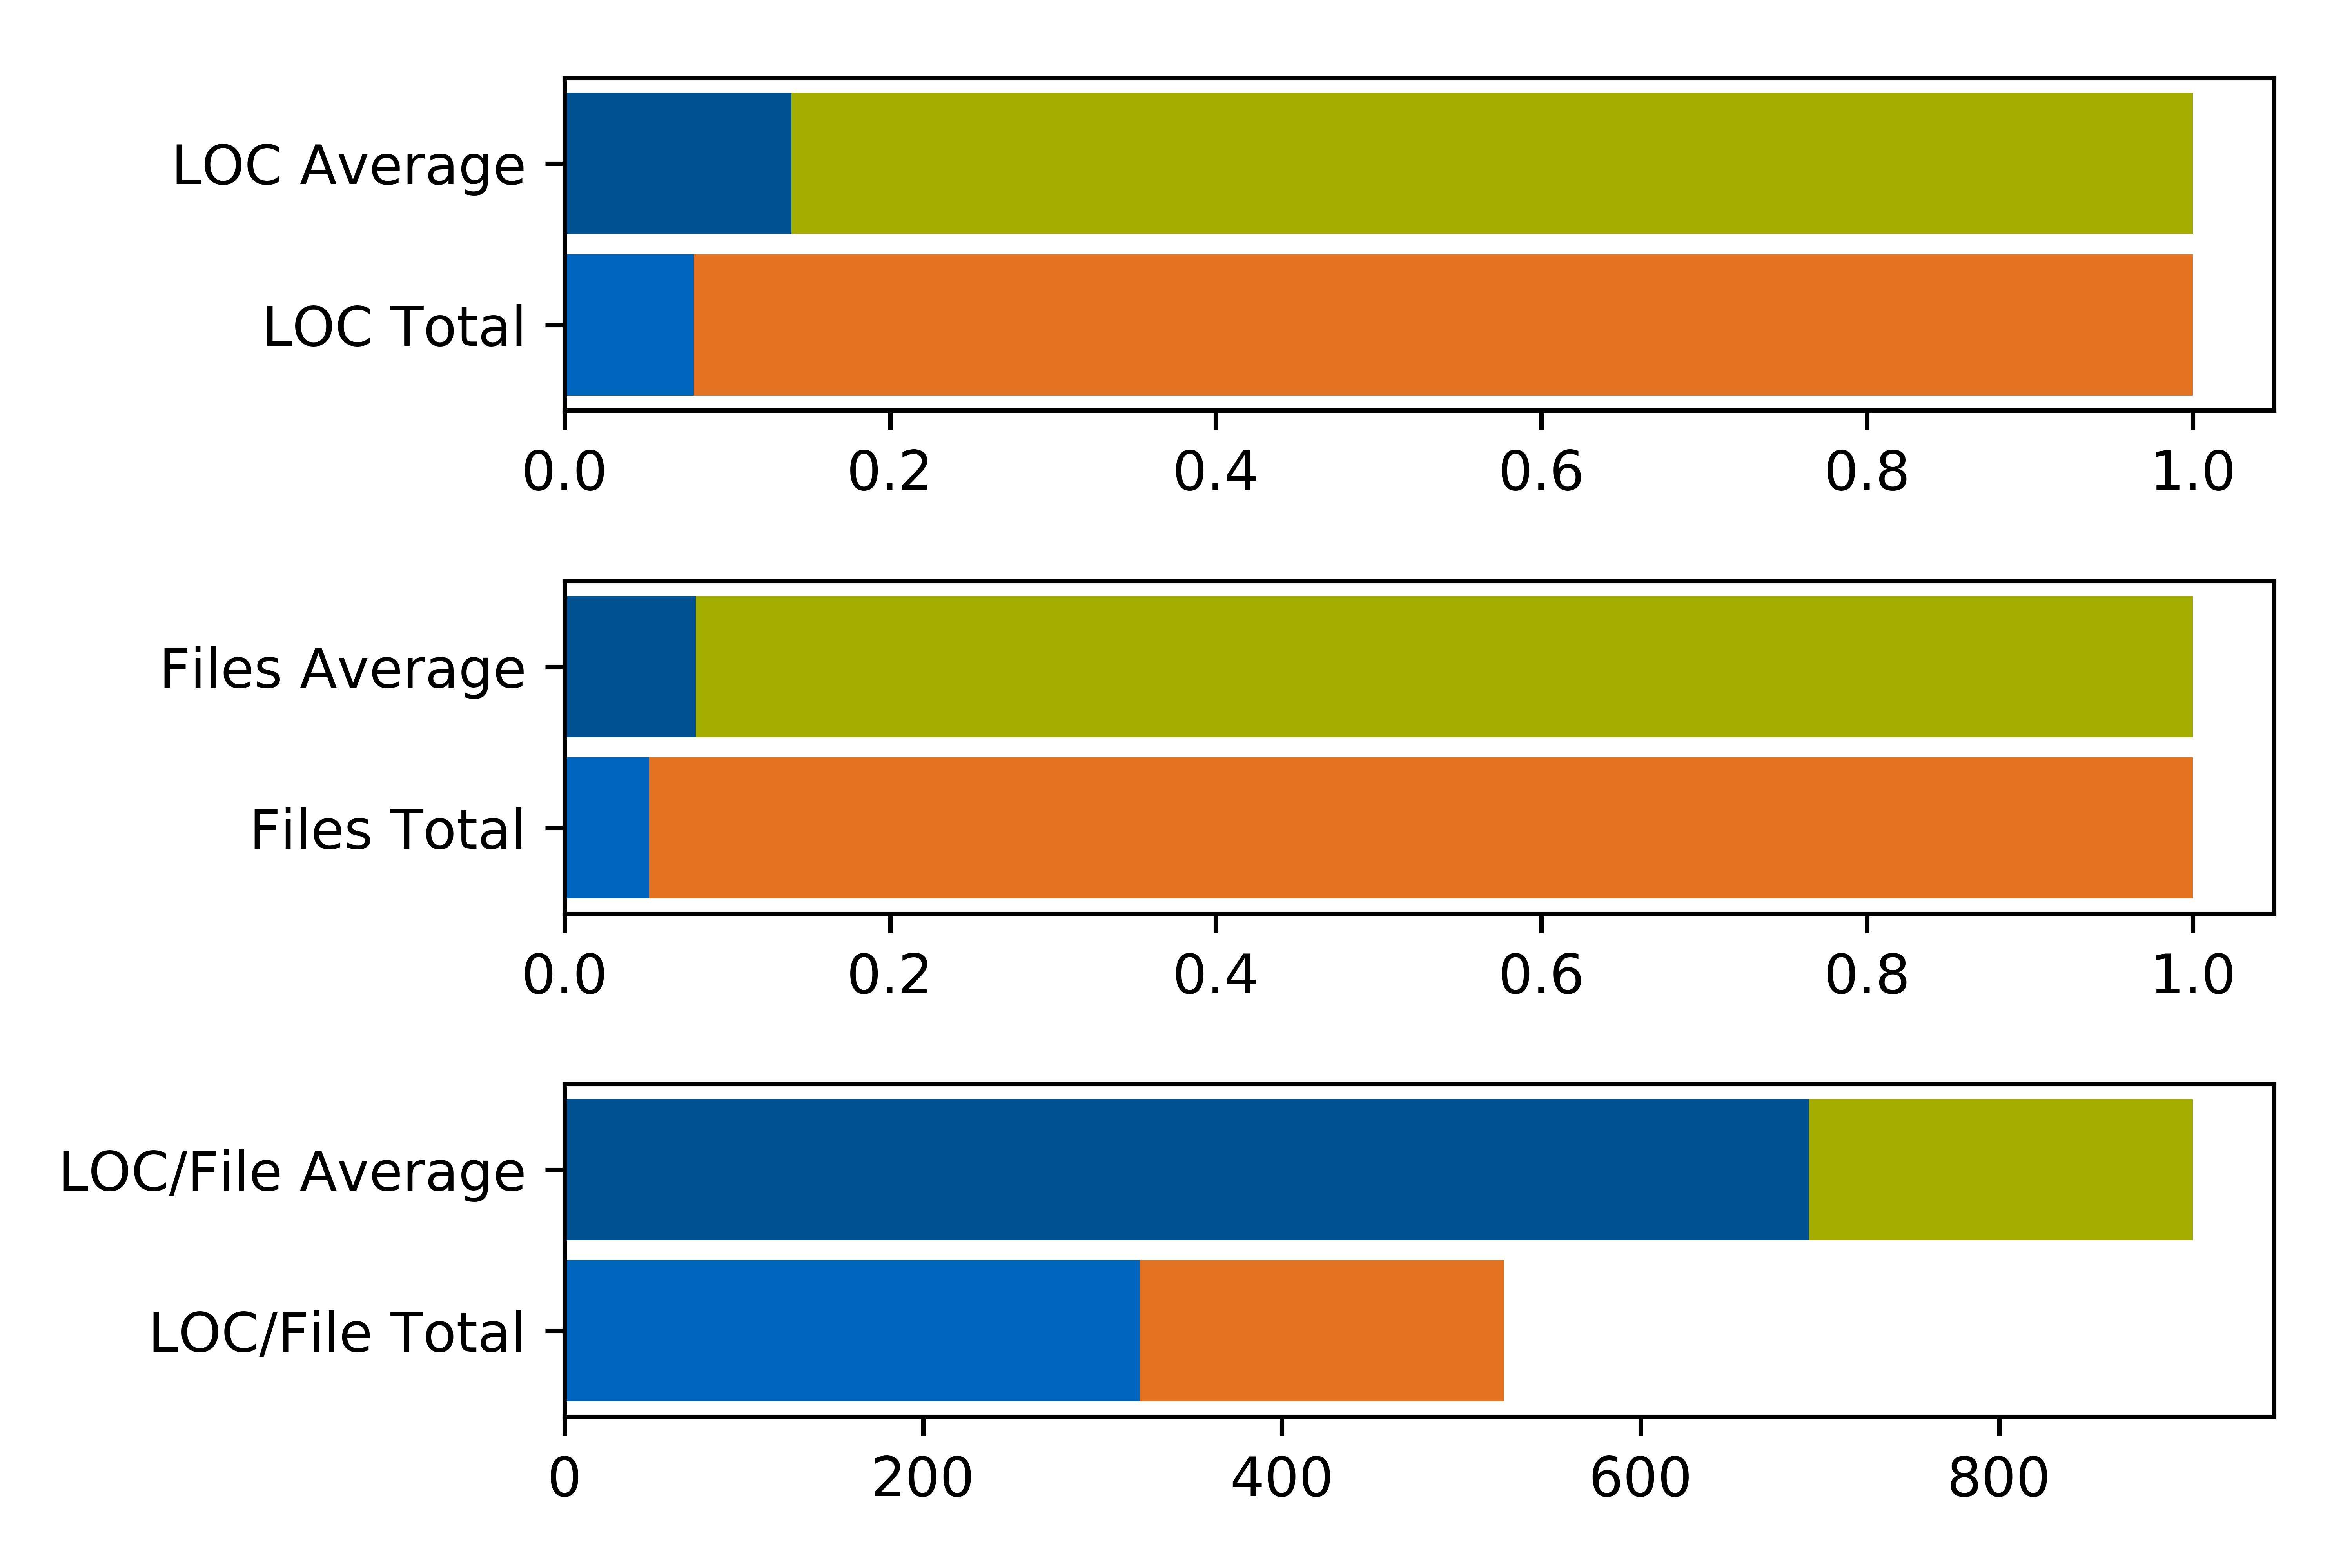
\includegraphics[width=\linewidth]{figures/QualitasCorpusComparison/comparison.png}
	\caption[Comparison of generated and manually maintained code in the Qualitas Corpus]{Comparison of generated and manually maintained code in the Qualitas Corpus.	Blue displays the generated proportion whereas green and orange display the manually maintained ones.
		}
	\label{fig:comparison}
\end{figure}

\subsubsection{Lines of code for generated and manually maintained source code.}
\label{section:qualitasCorpusLOC}
The Table~\ref{table:locQualitasCorpus} shows how many \textit{lines of code} fall into the categories of generated and manually maintained code augmented with the ratios the categories cover. The ratio in lines of code for generated source code range from very low values \textit{(0,05\% - Hibernate)} up to more than three fourth \textit{(75,03\% - Cobertura)} of the overall lines of code.\\
The average proportion of generated lines of code is calculated using the equation
\begin{equation}
	\label{eq:locAvg}
	LOC_{avg} = \frac{\mathlarger{\sum^{projects} \frac{LOC_{generated}}{LOC}}}{|projects|} = 13.95\%
\end{equation}
The total proportion of generated lines of code is calculated via
\begin{equation}
	\label{eq:locTotal}
	LOC_{total} = \frac{\mathlarger{\sum^{projects} LOC_{generated}}}{\mathlarger{\sum^{projects} LOC}} = 7.96\%
\end{equation} 
The average and total proportions of manually maintained lines of code are described by the complementary probability.

% !TeX root = ../main.tex
% Add the above to each chapter to make compiling the PDF easier in some editors.
\setlength{\extrarowheight}{-.17em}
\begin{table}
	\caption[Lines of code distributions in the Qualitas Corpus.]{The absolute and relative proportions of lines of code in the code categories generated and manually maintained in the Qualitas Corpus.}
	\label{table:locQualitasCorpus}
	\begin{tabularx}{\textwidth}{c|r|r|r|r|r}
		& \multicolumn{5}{c}{Lines of Code}  \\
		Project & All & \multicolumn{2}{c|}{Generated} & \multicolumn{2}{c}{Manually}  \\
		\hline
		argouml & 389.952 & 11.992 & 3,08\% & 377.960 & 96,92\% \\
		axion & 41.862 & 5.417 & 12,94\% & 36.445 & 87,06\% \\
		castor & 349.301 & 18.056 & 5,17\% & 331.245 & 94,83\% \\
		cayenne & 341.902 & 15.528 & 4,54\% & 326.374 & 95,46\% \\
		cobertura & 68.154 & 51.139 & 75,03\% & 17.015 & 24,97\% \\
		compiere & 727.702 & 206.999 & 28,45\% & 520.703 & 71,55\% \\
		derby & 1.138.858 & 46.974 & 4,12\% & 1.091.884 & 95,88\% \\
		eclipse\_SDK & 4.956.920 & 103.292 & 2,08\% & 4.853.628 & 97,92\% \\
		exoportal & 146.947 & 3.353 & 2,28\% & 143.594 & 97,72\% \\
		findbugs & 185.806 & 5.895 & 3,17\% & 179.911 & 96,83\% \\
		galleon & 135.442 & 4.888 & 3,61\% & 130.554 & 96,39\% \\
		gt2 & 1.514.789 & 325.259 & 21,47\% & 1.189.530 & 78,53\% \\
		hadoop & 444.593 & 9.475 & 2,13\% & 435.118 & 97,87\% \\
		hibernate & 711.370 & 327 & 0,05\% & 711.043 & 99,95\% \\
		hsqldb & 269.978 & 1.100 & 0,41\% & 268.878 & 99,59\% \\
		ireport & 338.819 & 100.276 & 29,60\% & 238.543 & 70,40\% \\
		jag & 28.957 & 10.326 & 35,66\% & 18.631 & 64,34\% \\
		jasperreports & 347.502 & 4.978 & 1,43\% & 342.524 & 98,57\% \\
		javacc & 35.145 & 8.509 & 24,21\% & 26.636 & 75,79\% \\
		jboss & 968.808 & 8.173 & 0,84\% & 960.635 & 99,16\% \\
		jchempaint & 372.743 & 386 & 0,10\% & 372.357 & 99,90\% \\
		jedit & 176.672 & 9.575 & 5,42\% & 167.097 & 94,58\% \\
		jena & 164.679 & 5.045 & 3,06\% & 159.634 & 96,94\% \\
		jhotdraw & 133.830 & 17.062 & 12,75\% & 116.768 & 87,25\% \\
		jparse & 32.270 & 20.738 & 64,26\% & 11.532 & 35,74\% \\
		jrefactory & 301.940 & 46.449 & 15,38\% & 255.491 & 84,62\% \\
		jruby & 244.774 & 4.033 & 1,65\% & 240.741 & 98,35\% \\
		jstock & 74.361 & 30.446 & 40,94\% & 43.915 & 59,06\% \\
		lucene & 611.422 & 60.330 & 9,87\% & 551.092 & 90,13\% \\
		mvnforum & 172.855 & 32.103 & 18,57\% & 140.752 & 81,43\% \\
		myfaces\_core & 189.954 & 19.678 & 10,36\% & 170.276 & 89,64\% \\
		netbeans & 7.142.778 & 688.961 & 9,65\% & 6.453.817 & 90,35\% \\
		pmd & 80.971 & 27.671 & 34,17\% & 53.300 & 65,83\% \\
		poi & 363.487 & 21.621 & 5,95\% & 341.866 & 94,05\% \\
		sablecc & 35.388 & 21.134 & 59,72\% & 14.254 & 40,28\% \\
		struts & 261.537 & 6.978 & 2,67\% & 254.559 & 97,33\% \\
		tomcat & 352.572 & 7.356 & 2,09\% & 345.216 & 97,91\% \\
		velocity & 70.804 & 9.092 & 12,84\% & 61.712 & 87,16\% \\
		wct & 99.622 & 150 & 0,15\% & 99.472 & 99,85\% \\
		weka & 496.737 & 5.132 & 1,03\% & 491.605 & 98,97\% \\
		xalan & 354.578 & 3.217 & 0,91\% & 351.361 & 99,09\% \\
	\end{tabularx}
\end{table}
\setlength{\extrarowheight}{0em}

\subsubsection{Number of generated and manually maintained source code files.}
Table~\ref{table:countQualitasCorpus} additionally displays the \textit{number of source code files} that are generated next to the ones that are manually maintained. The ratios the code categories cover are again associated to the absolute values, whereas they range from a very small amount of files \textit{(0,02\% - Hibernate)} up to around two third \textit{(68,18\% - SableCC)}.\\
Analog to the calculation of the total and the average ratios of generated to manually maintained lines of code as described in in Section~\ref{section:qualitasCorpusLOC} are the proportions of generated to manually maintained files calculated. The same equations~\ref{eq:locAvg}~and~\ref{eq:locTotal} are used, but LOC is replaced by the number of files. %Figure~\ref{fig:comparison} displays the ratios.\\
This resulted in the proportions of generated files of
\begin{equation}
	Files_{avg} = 8.07\%, \quad Files_{total} = 5.19\%
\end{equation} 
Again, the average and total proportions of manually maintained files are described by the complementary probability.

% !TeX root = ../main.tex
% Add the above to each chapter to make compiling the PDF easier in some editors.
\setlength{\extrarowheight}{-.15em}
\begin{table}
	\caption{The results our algorithm has created.}
	\label{table:countQualitasCorpus}
	\begin{tabularx}{\textwidth}{c|c|c|c|c|c}
		 & \multicolumn{5}{c}{Source code files}  \\
		Project & All & \multicolumn{2}{c|}{Generated} & \multicolumn{2}{c}{Manually}\\
		\hline
		argouml & 1.922 & 3 & 0,16\% & 1.919 & 99,84\% \\
		axion & 237 & 7 & 2,95\% & 230 & 97,05\% \\
		castor & 2.229 & 61 & 2,74\% & 2.168 & 97,26\% \\
		cayenne & 2.796 & 227 & 8,12\% & 2.569 & 91,88\% \\
		cobertura & 140 & 34 & 24,29\% & 106 & 75,71\% \\
		compiere & 2.508 & 681 & 27,15\% & 1.827 & 72,85\% \\
		derby & 2.842 & 17 & 0,60\% & 2.825 & 99,40\% \\
		eclipse\_SDK & 22.263 & 235 & 1,06\% & 22.028 & 98,94\% \\
		exoportal & 1.839 & 23 & 1,25\% & 1.816 & 98,75\% \\
		findbugs & 1.062 & 7 & 0,66\% & 1.055 & 99,34\% \\
		galleon & 255 & 19 & 7,45\% & 236 & 92,55\% \\
		gt2 & 7.097 & 1.493 & 21,04\% & 5.604 & 78,96\% \\
		hadoop & 1.988 & 14 & 0,70\% & 1.974 & 99,30\% \\
		hibernate & 6.214 & 1 & 0,02\% & 6.213 & 99,98\% \\
		hsqldb & 514 & 1 & 0,19\% & 513 & 99,81\% \\
		ireport & 1.626 & 235 & 14,45\% & 1.391 & 85,55\% \\
		jag & 132 & 20 & 15,15\% & 112 & 84,85\% \\
		jasperreports & 1.589 & 10 & 0,63\% & 1.579 & 99,37\% \\
		javacc & 195 & 40 & 20,51\% & 155 & 79,49\% \\
		jboss & 6.806 & 199 & 2,92\% & 6.607 & 97,08\% \\
		jchempaint & 2.042 & 5 & 0,24\% & 2.037 & 99,76\% \\
		jedit & 531 & 11 & 2,07\% & 520 & 97,93\% \\
		jena & 914 & 18 & 1,97\% & 896 & 98,03\% \\
		jhotdraw & 613 & 67 & 10,93\% & 546 & 89,07\% \\
		jparse & 75 & 7 & 9,33\% & 68 & 90,67\% \\
		jrefactory & 2.229 & 140 & 6,28\% & 2.089 & 93,72\% \\
		jruby & 1.128 & 9 & 0,80\% & 1.119 & 99,20\% \\
		jstock & 274 & 52 & 18,98\% & 222 & 81,02\% \\
		lucene & 3.036 & 89 & 2,93\% & 2.947 & 97,07\% \\
		mvnforum & 705 & 100 & 14,18\% & 605 & 85,82\% \\
		myfaces\_core & 1.052 & 60 & 5,70\% & 992 & 94,30\% \\
		netbeans & 32.567 & 1.864 & 5,72\% & 30.703 & 94,28\% \\
		pmd & 751 & 162 & 21,57\% & 589 & 78,43\% \\
		poi & 2.007 & 14 & 0,70\% & 1.993 & 99,30\% \\
		sablecc & 198 & 135 & 68,18\% & 63 & 31,82\% \\
		struts & 1.836 & 43 & 2,34\% & 1.793 & 97,66\% \\
		tomcat & 1.324 & 44 & 3,32\% & 1.280 & 96,68\% \\
		velocity & 371 & 9 & 2,43\% & 362 & 97,57\% \\
		wct & 638 & 1 & 0,16\% & 637 & 99,84\% \\
		weka & 1.271 & 9 & 0,71\% & 1.262 & 99,29\% \\
		xalan & 975 & 2 & 0,21\% & 973 & 99,79\% \\
	\end{tabularx}
\end{table}
\setlength{\extrarowheight}{0em}

\subsubsection{Lines of code per source code file}
When looking at the Tables~\ref{table:countQualitasCorpus}~and~\ref{table:locQualitasCorpus} we saw that in many projects only a few generated files are responsible for a high number in lines of code.\\
We decided to calculate the proportion of lines of code per file for the generated and the manually maintained files and could confirm that there exists indeed a correlation between the file size and the possible generation as stated in~\cite{Bernwieser2014}.\\
We calculated a \textbf{total} ratio of generated lines of code to generated files of 
\begin{equation}
	\frac{LOC_{generated}}{Files_{generated}} = 321 , \quad \frac{LOC_{manually}}{Files_{manually}} = 204
\end{equation}
and an \textbf{average} ratio of
\begin{equation}
	\frac{LOC_{generated}}{Files_{generated}} = 694 , \quad \frac{LOC_{manually}}{Files_{manually}} = 214
\end{equation}

\subsection{Random Git Projects}
We started the search for generated code in the huge, randomly composed collection of open source projects by again applying the algorithm created for this thesis. In the first iteration we filtered the source code files using the generator-patterns found in the Qualitas Corpus. In the second iteration we used all generator-patterns found in the collection. \\
The Tables~\ref{table:locGit} and~\ref{table:countGit} show the results of the first and the second iteration. The column \textit{Only Qualitas Corpus} refers to the first iteration using only the generator-patterns found in the Qualitas Corpus to filter the files. The column \textit{Git Patterns added} describes the second iteration using all patterns found in the open source projects.

\subsubsection{Number of generator-patterns found}
We found a total of 34 new generator patterns that are widely distributed over the different programming languages. These are again regular expressions that accept a multitude of different patterns so that the final number of found generator patterns is much higher.

\subsubsection{Lines of code for generated and manually maintained source code.}
Table~\ref{table:locGit} shows the results for the generated lines of code gathered during the two iteration steps.\\
In the first iteration the proportion of generated lines of code range from 0.01\% for the Swift projects up to 8.88\% for the Java projects. This result can be explained as the Qualitas Corpus contains only projects written in Java, so the previously found generator-patterns do apply best for the Java projects. Nonetheless some of the patterns are universal and are created by code generators that are able to generate code for different programming languages.\\
The total and average proportions for the lines of code are calculated analog to the procedure for the Qualitas Corpus and result in
\footnote{
	\label{note:onlyGenerated}
	We include only the projects that do contain generated code so the results are better comparable to the ones gathered for the Qualitas Corpus.
}:
\begin{equation}
	\label{eq:locGit_1}
	LOC_{avg} = 2.60\%, \quad LOC_{total} = 3.23\%
\end{equation}
Again, the average and total proportions of manually maintained files are described by the complementary probability.
In the second iteration the proportion of generated code found by using the patterns included in the collection raises enormously. Especially in the projects not written in Java the amount of detected generated code is utterly enlarged.\\
Again we calculated the total and average proportions and found the following\footref{note:onlyGenerated}:
\begin{equation}
\label{eq:locGit_2}
LOC_{avg} = 17.66\%, \quad LOC_{total} = 12.88\%
\end{equation}
Again, the average and total proportions of manually maintained files are described by the complementary probability.
% !TeX root = ../main.tex
% Add the above to each chapter to make compiling the PDF easier in some editors.
\setlength{\extrarowheight}{-.0em}
\begin{table}
		\caption[Lines of code distributions in the collection of open source projects.]{The absolute and relative proportions of lines of code in the code categories generated and manually maintained in the collection of open source projects.}
	\label{table:locGit}
	\begin{tabularx}{\textwidth}{c|c|c|c|c|c}
		& \multicolumn{5}{c}{Lines of Code}  \\
		Project & All & \multicolumn{2}{c|}{Only Qualitas Corpus} & \multicolumn{2}{c}{Git Patterns added}  \\
		\hline
		ABAP & 55.498 & 0 & 0,00\% & 0 & 0,00\% \\
		Ada & 194.961 & 0 & 0,00\% & 42.312 & 21,70\% \\
		C & 4.791.612 & 117.033 & 2,44\% & 402.644 & 8,40\% \\
		COBOL & 58.968 & 0 & 0,00\% & 0 & 0,00\% \\
		Delphi & 15.470 & 0 & 0,00\% & 0 & 0,00\% \\
		Gosu & 2.738 & 0 & 0,00\% & 0 & 0,00\% \\
		Groovy & 143.939 & 0 & 0,00\% & 386 & 0,27\% \\
		Java & 4.879.454 & 433.357 & 8,88\% & 687.973 & 14,10\% \\
		JavaScript & 6.828.723 & 27.151 & 0,40\% & 323.986 & 4,74\% \\
		Kotlin & 87.132 & 0 & 0,00\% & 15.586 & 17,89\% \\
		Matlab & 134.229 & 0 & 0,00\% & 0 & 0,00\% \\
		OScript & 2.837.202 & 86.852 & 3,06\% & 449.116 & 15,83\% \\
		PHP & 1.016.013 & 8.214 & 0,81\% & 191.794 & 18,88\% \\
		Python & 858.223 & 0 & 0,00\% & 284.733 & 33,18\% \\
		Rust & 1.248.308 & 0 & 0,00\% & 17.795 & 1,43\% \\
		Swift & 457.629 & 52 & 0,01\% & 264.650 & 57,83\% \\
		XML & 28.541 & 0 & 0,00\% & 0 & 0,00\% \\		
	\end{tabularx}
\end{table}
\setlength{\extrarowheight}{0em}

\subsubsection{Number of generated and manually maintained source code files.}
Table~\ref{table:countGit} shows the results for the generated lines of code gathered during the two iteration steps.\\
The total and average proportions for the amount of generated source code files are again calculated using the equations used for the Qualitas Corpus.
For the first iteration this results in the proportions of generated files of
\begin{equation}
\label{eq:countGit_1}
	Files_{avg} = 1.32\%, \quad Files_{total} = 2.15\%
\end{equation} 
For the second iterations the results are 
\begin{equation}
\label{eq:countGit_2}
Files_{avg} = 8.97\%, \quad Files_{total} = 8.68\%
\end{equation} 
% !TeX root = ../main.tex
% Add the above to each chapter to make compiling the PDF easier in some editors.
\setlength{\extrarowheight}{-.0em}
\begin{table}
	\caption[Source code file distributions in the collection of open source projects.]{The absolute and relative proportions of source code files in the code categories generated and manually maintained in the collection of open source projects. }
	\label{table:countGit}
	\begin{tabularx}{\textwidth}{c|c|c|c|c|c}
		 & \multicolumn{5}{c}{Source code files}  \\
		Project & All & \multicolumn{2}{c|}{Only Qualitas Corpus} & \multicolumn{2}{c}{Git Patterns added}  \\
		\hline
		ABAP & 228 & 0 & 0,00\% & 0 & 0,00\% \\
		Ada & 1.433 & 0 & 0,00\% & 232 & 16,19\% \\
		C & 11.108 & 19 & 0,17\% & 265 & 2,39\% \\
		COBOL & 161 & 0 & 0,00\% & 0 & 0,00\% \\
		Delphi & 15 & 0 & 0,00\% & 0 & 0,00\% \\
		Gosu & 15 & 0 & 0,00\% & 0 & 0,00\% \\
		Groovy & 1.499 & 0 & 0,00\% & 4 & 0,27\% \\
		Java & 32.573 & 1.522 & 4,67\% & 2.971 & 9,12\% \\
		JavaScript & 25.461 & 6 & 0,02\% & 347 & 1,36\% \\
		Kotlin & 929 & 0 & 0,00\% & 106 & 11,41\% \\
		Matlab & 1.408 & 0 & 0,00\% & 0 & 0,00\% \\
		OScript & 18.076 & 481 & 2,66\% & 2.462 & 13,62\% \\
		PHP & 4.847 & 16 & 0,33\% & 1.344 & 27,73\% \\
		Python & 3.035 & 0 & 0,00\% & 204 & 6,72\% \\
		Rust & 3.636 & 0 & 0,00\% & 26 & 0,72\% \\
		Swift & 2.638 & 2 & 0,08\% & 1.173 & 44,47\% \\
		XML & 195 & 0 & 0,00\% & 0 & 0,00\% \\		
	\end{tabularx}
\end{table}
\setlength{\extrarowheight}{0em}

\subsubsection{Lines of code per source code file}
As a last point concerning the open source projects we calculated again the ratio of lines of code per source code file for the two iterations.\\
In the first iteration we found the total ratios of of:
\begin{equation}
	\frac{LOC_{generated}}{Files_{generated}} = 329 , \quad \frac{LOC_{manually}}{Files_{manually}} = 217
\end{equation}
and an \textbf{average} ratio of
\begin{equation}
	\frac{LOC_{generated}}{Files_{generated}} = 1948 , \quad \frac{LOC_{manually}}{Files_{manually}} = 228
\end{equation}
In the second iteration the ratios changed to:
\begin{equation}
\frac{LOC_{generated}}{Files_{generated}} = 293 , \quad \frac{LOC_{manually}}{Files_{manually}} = 215
\end{equation}
and an \textbf{average} ratio of
\begin{equation}
\frac{LOC_{generated}}{Files_{generated}} = 522 , \quad \frac{LOC_{manually}}{Files_{manually}} = 198
\end{equation}

\section{Discussion}
By analyzing the projects included in the Qualitas Corpus we found a wide variety of generator-patterns and were able to calculate the average and total proportions of generated to manually maintained lines of code and files. We saw that generated code makes only a small portion of the all lines of code, whereas in average a project contains 13.95\% generated lines of code and all projects contained 7.96\% generated lines of code.\\
Additionally we saw that in average 8.07\% of files are generated whereas in total only 5.19\% are generated.\\
We were able to find even more generator-patterns and resulting a higher number of generated source code after applying the algorithm on the huge set of open source projects. Hereby we found that the projects do contain even more generated code with a total of 12.88\% and an average of 17.66\% of the lines of code being generated. Also the total amount of files has risen to 8.97\% and the total amount to 8.68\%.\\
Resulting from that we showed that in average the generated files always contain more lines of code than the manually maintained ones, whereas there exists no direct correlation of the actual lines of code ratios between generated and manually maintained source code files.

\subsection{Completeness and accuracy}
We found the generator-patterns by iterating over the Qualitas Corpus and applying the algorithm described in Chapter~\ref{chapter:approach}. The found patterns had been added to the generator-pattern repository and used to filter all files that we were able to classify as generated in the next iteration.\\
In every iteration the amount of possible generator-patterns could be lowered by using this technique very fast until all generator-patterns were reviewed by hand and so all patterns had been found in the Qualitas Corpus.\\
We compared our results to these described in \cite{Bernwieser2014} and could confirm that our approach found all files and even. Resulting from this we concluded that our approach is as complete as it can be using the technique of suffix-tree clone-detection on the comments.\\
By using the approach on the huge random collection of open source projects we detected some more generator-patterns that were not included in the Qualitas Corpus. Nonetheless we were able to filter many generated files in the first iteration by using the generator-pattern repository what supports our assertion that the algorithm found all generator patterns that were included in the Qualitas Corpus.\\
Additionally, the generator-pattern repository is easily extendable with new patterns at any time what was shown by applying the algorithm on the collection of open source projects. So by gradually extending the repository by applying the suffix-tree clone-detection approach on the comments, the repository will saturate with patterns and will over time become complete and highly accurate in terms of generator-patterns.

\subsection{Relevance of results}

\annotation{Not sure what to write in this section.\\ Maybe how the generator-pattern repository can be used by Teamscale to lower amount of work done in analysis by excluding the generated files?}

\section{Threats to validity}
This section describes the threads that may have an impact on the validity of the results generated by our approach and justifies how .
\subsection{Wrong filtering}
In Step~\ref{section:filterCloneResults} we used the regular expression shown in Listing~\ref{lst:generatorPattern}. This reduces the amount of resulting \code{CloneResult}s to a level that can be processed by a human. Our observations showed that indeed most of the generator-patterns contained the regex so that it can be considered as only a small thread.\\
Nonetheless did we found generator-patterns that didn't contain the regex. These patterns make only a very small portion of all generator-patterns so we didn't see a value in refining it. Furthermore does step~\ref{section:generateLinks} also save files and links for the not generated found \code{CloneClass}es that can be reviewed in addition to the generated ones. The problem arising is that the amount of data to review is way to high as i could be process by hand, but the ones that had the highest number of occurrences were also searched by us what revealed the patterns that didn't include the regular expression.\\
In conclusion we can say that the regular expression is a very good filter to find the generator-patterns which can be easily extended to also review the patterns that were filtered out to find all generator-patterns.

\subsection{Minimum clone length vs. irrelevant data}
We faced the decision on a most optimal minimum clone length while applying the suffix-tree clone-detection algorithm made by Esko Ukkonen~\cite{Ukkonen1995} and the search for clones on the resulting tree structure. We finally decided on a length of 5. \\
The draw-off we faced was the one that a high minimum clone length resulted in a low number of \code{CloneResult}s. Hereby were all short generator-patterns sorted out before we were even aware that they existed in the code base.\\
On the other hand was a low minimum clone length not really much applicable due to the fact that it generated really much false positives like only the words \textit{generated, modify, edit}, whereas they do not hold any value without the context they were used in. Especially the word generated is often used in the context that the following method generates some sort of date, not that the method itself is generated.\\
Therefore we did a benchmark iterating over the minimum clone length and comparing the amount of data the different lengths generated and the subjective observation how useful the data was. In Figures~\ref{fig:thresholdsAll} we saw that the unfiltered \code{CloneResult}s do follow a nearly exponential descend, whereas a the minimum clone length of 5 creates only around 15\% compared to a length of 2. This arises the question whether a minimum clone length of 5 erases to much valuable data.\\
When you look at Figure~\ref{fig:thresholdsProcessed} we saw that by applying the three processing steps of filtering by the regular expression described in Step~\ref{section:filterCloneResults}, then accumulating the \code{CloneResult}s as stated in Step~\ref{section:accumulation} and finally clustering the results explained in Step~\ref{section:clustering} resulted in an amount of found \code{CloneResult}s having it's peak at the minimum clone length of 3. Nonetheless we decided on a length of 5 due to the fact that it erases only around 20\% in the final presumable generator-patterns generated, but it generates patterns that are much more speaking for themselves due to the extended length.\\
Additionally, we saw that the patterns which are lost by increasing the minimum clone length up to the length of 5 are all included in the patterns we found also by using the higher length. This is due to the fact that the shorter presumable patterns do overlap with the patterns found with the length of 5, but are no direct substrings of the longer generator-patterns. Nonetheless they do point to the same classes and in fact to the same patterns.\\
Following these thoughts we found the decided on a minimum clone length of 5.

\subsection{Representativeness of data sets}
We used the Qualitas Corpus as a reference set because it is declared as "intended to be used for empirical studies of code artefacts. The primary goal is to provide a resource that supports reproducible studies of software" \cite{TemperoEwanandAnslowCraigandDietrichJensandHanTedandLiJingandLumpeMarkusandMeltonHaydenandNoble2010a}. It is used in a variety of other studies and the results can be easily compared.\\
As we showed it includes a high number of generated code and also many generator-patterns, what makes it a good starting point to begin working with the created algorithm. Furthermore it consists of a high number of different projects (112) that are all maintained by big software companies and used in production. Due to the fact that \textit{CQSE GmbH} and their product \textit{Teamscale} is mostly used by big international companies to monitor their code quality, the parallels found between the projects led us to the conclusion that the Qualitas Corpus is a good starting point for the use in \textit{Teamscale}.\\
Nonetheless the problem we see in using the Qualitas Corpus is that it consists only of projects written in Java, which makes it only representative for this particular programming language. To avoid this problem we additionally used the algorithm on a huge randomly composed collection of open source projects we gathered from \href{github.com}{GitHub} we made a second, wide spread reference dataset developed by a huge number of independent programmers. This dataset is composed of very small up to really big projects that are written in a multitude of programming languages and developed all around the globe.\\
This led us to the conclusion that in conjunction the two reference datasets give a representative profile of very much, very different projects that are all developed under very unique circumstances.

\subsection{Generators without pattern}
A last thread we are facing is that there exists also a multitude of code generators that do not mark their artifacts with a characteristic pattern in the comments. Especially custom written generators often don't add a generator pattern.\\
This problem can't be faced with the current approach of suffix-tree clone-detection on the comments. To find these generated artifacts one has to combine our approach with e.g. the one described in \cite{Bernwieser2014}.